\documentclass[landscape,final,a0paper]{baposter}
\tracingstats=2

\usepackage{url}
\usepackage{calc}
\usepackage{graphicx}
\usepackage{amsmath}
\usepackage{amssymb}
\usepackage{relsize}
\usepackage{multirow}
\usepackage{bm}

\usepackage{graphicx}
\usepackage{multicol}

\usepackage{pgfbaselayers}
\pgfdeclarelayer{background}
\pgfdeclarelayer{foreground}
\pgfsetlayers{background,main,foreground}

\usepackage{times}
\usepackage{helvet}
\usepackage{palatino}

\newcommand{\captionfont}{\footnotesize}

\selectcolormodel{cmyk}

%\graphicspath{{images/}}

%%%%%%%%%%%%%%%%%%%%%%%%%%%%%%%%%%%%%%%%%%%%%%%%%%%%%%%%%%%%%%%%%%%%%%%%%%%%%%%%
%%%% Some math symbols used in the text
%%%%%%%%%%%%%%%%%%%%%%%%%%%%%%%%%%%%%%%%%%%%%%%%%%%%%%%%%%%%%%%%%%%%%%%%%%%%%%%%
% Format 

\renewcommand{\Pr}{\mbox{P}}
\newcommand{\e}{\mbox{e}}
\newcommand{\dx}{\,\mbox{d}x}

%%%%%%%%%%%%%%%%%%%%%%%%%%%%%%%%%%%%%%%%%%%%%%%%%%%%%%%%%%%%%%%%%%%%%%%%%%%%%%%%
% Multicol Settings
%%%%%%%%%%%%%%%%%%%%%%%%%%%%%%%%%%%%%%%%%%%%%%%%%%%%%%%%%%%%%%%%%%%%%%%%%%%%%%%%
\setlength{\columnsep}{0.7em}
\setlength{\columnseprule}{0mm}


%%%%%%%%%%%%%%%%%%%%%%%%%%%%%%%%%%%%%%%%%%%%%%%%%%%%%%%%%%%%%%%%%%%%%%%%%%%%%%%%
% Save space in lists. Use this after the opening of the list
%%%%%%%%%%%%%%%%%%%%%%%%%%%%%%%%%%%%%%%%%%%%%%%%%%%%%%%%%%%%%%%%%%%%%%%%%%%%%%%%
\newcommand{\compresslist}{%
\setlength{\itemsep}{1pt}%
\setlength{\parskip}{0pt}%
\setlength{\parsep}{0pt}%
}


%%%%%%%%%%%%%%%%%%%%%%%%%%%%%%%%%%%%%%%%%%%%%%%%%%%%%%%%%%%%%%%%%%%%%%%%%%%%%%
%%% Begin of Document
%%%%%%%%%%%%%%%%%%%%%%%%%%%%%%%%%%%%%%%%%%%%%%%%%%%%%%%%%%%%%%%%%%%%%%%%%%%%%%

\begin{document}

%%%%%%%%%%%%%%%%%%%%%%%%%%%%%%%%%%%%%%%%%%%%%%%%%%%%%%%%%%%%%%%%%%%%%%%%%%%%%%
%%% Here starts the poster
%%%---------------------------------------------------------------------------
%%% Format it to your taste with the options
%%%%%%%%%%%%%%%%%%%%%%%%%%%%%%%%%%%%%%%%%%%%%%%%%%%%%%%%%%%%%%%%%%%%%%%%%%%%%%
% Define some colors
\definecolor{silver}{cmyk}{0,0,0,0.3}
\definecolor{yellow}{cmyk}{0,0,0.9,0.0}
\definecolor{reddishyellow}{cmyk}{0,0.22,1.0,0.0}
\definecolor{black}{cmyk}{0,0,0.0,1.0}
\definecolor{darkYellow}{cmyk}{0,0,1.0,0.5}
\definecolor{darkSilver}{cmyk}{0,0,0,0.1}
\definecolor{lightyellow}{cmyk}{0,0,0.3,0.0}
\definecolor{lighteryellow}{cmyk}{0,0,0.1,0.0}
\definecolor{lighteryellow}{cmyk}{0,0,0.1,0.0}
\definecolor{lightestyellow}{cmyk}{0,0,0.05,0.0}
\definecolor{cyan}{cmyk}{1,0,0,0}
\definecolor{lightcyan}{cmyk}{0.5,0,0,0}
\definecolor{pastelcyan}{cmyk}{0.25,0,0,0}
\definecolor{magenta}{cmyk}{0,1,0,0}
\definecolor{yellow}{cmyk}{0,0,1,0}
\definecolor{lightyellow}{cmyk}{0,0,0.5,0}
\definecolor{pastelyellow}{cmyk}{0,0,0.25,0}
\definecolor{black}{cmyk}{0,0,0,1}
\definecolor{darkgray}{cmyk}{0,0,0,0.75}
\definecolor{gray}{cmyk}{0,0,0,0.5}
\definecolor{lightgray}{cmyk}{0,0,0,0.25}
\definecolor{white}{cmyk}{0,0,0,0}
\definecolor{red}{cmyk}{0,1,1,0}
\definecolor{orange}{cmyk}{0,0.5,1,0}
\definecolor{scarlet}{cmyk}{0,1,0.5,0}
\definecolor{brown}{cmyk}{0.5,0.75,1,0}
\definecolor{camel}{cmyk}{0.25,0.375,0.5,0}
\definecolor{cream}{cmyk}{0,0.2,0.3,0}
\definecolor{green}{cmyk}{1,0,1,0}
\definecolor{lightgreen}{cmyk}{0.5,0,0.5,0}
\definecolor{pastelgreen}{cmyk}{0.25,0,0.25,0}
\definecolor{mossgreen}{cmyk}{0.64,0.4,1,0}
\definecolor{yellowgreen}{cmyk}{0.5,0,1,0}
\definecolor{skyblue}{cmyk}{0.4,0.16,0,0}
\definecolor{royal}{cmyk}{1.0,0.5,0,0}
\definecolor{navyblue}{cmyk}{0.9,0.75,0.5,0}
\definecolor{lightnavy}{cmyk}{0.4,0.3,0.2,0}
\definecolor{blue}{cmyk}{1,1,0,0}
\definecolor{lightblue}{cmyk}{0.5,0.5,0,0}
\definecolor{pastelblue}{cmyk}{0.25,0.25,0,0}
\definecolor{lightpastelblue}{cmyk}{0.15,0.15,0,0}
\definecolor{lightestpastelblue}{cmyk}{0.05,0.05,0,0}
\definecolor{lavender}{cmyk}{0.25,0.25,0,0}
\definecolor{violet}{cmyk}{0.75,1,0.25,0}
\definecolor{purple}{cmyk}{0.5,1,0.5,0}
\definecolor{lightpurple}{cmyk}{0.25,0.5,0.25,0}
\definecolor{pink}{cmyk}{0,0.5,0,0}


%%

\typeout{Poster Starts}
%\background{
  %\begin{tikzpicture}[remember picture,overlay]%
  %  \draw (current page.north west)+(-2em,-2em) node[anchor=north west] %{\hspace{-2em}\includegraphics[height=1.1\textheight]{silhouettes_background}};
 % \end{tikzpicture}%
%}




\newlength{\leftimgwidth}
\begin{poster}%
  % Poster Options, such as colours etc
  {
  % Show grid to help with alignment
  grid=false,
 % Column spacing
  colspacing=0.5em,
 % Color style
 % bgColorOne=pastelblue,
 %bgColorTwo=lightpastelblue,
  bgColorOne=white,
  bgColorTwo=white,
  borderColor=darkgreen,
  headerColorOne=lightgreen,
  headerColorTwo=purple,
  headerFontColor=black,
 % boxColorOne=lightpastelblue,
 % boxColorTwo=lightestpastelblue,
 boxColorOne=white,
 boxColorTwo=white,
 % Format of textbox
  textborder=roundedleft,
% textborder=rectangle,
% Format of text header
  eyecatcher=true,
  headerborder=open,
  headerheight=0.10\textheight,
  headershape=roundedright,
  headershade=plain,
  headerfont=\Large\textsf, %Sans Serif
  boxshade=plain,
%  background=shade-tb,
 % background=plain,
  background=none,
  linewidth=2pt
  }
  % Eye Catcher
  {\includegraphics[width=10em]{imperial.pdf}} % select eyecatcher=false above if not required. If no eye catcher is present, the title is left aligned.
  % Title
  {\sf %Sans Serif
  %\bf% Serif
  Death ratio of COVID—19 \ with individual characteristics }
  % Authors
  {\sf %Sans Serif
  % Serif
  \vspace{1em} 
	JIAQI LI\\
	{\smaller Oral:  \url{https://imperial.cloud.panopto.eu/Panopto/Pages/Viewer.aspx?id=c40fac02-7068-4e89-b826-abd8006e8716}}
  }
  % University logo
  { % The makebox allows the title to flow into the logo
    \makebox[8em][r]{%
        \begin{minipage}{13em}
				\hfill \includegraphics[height=3em]{imperial.pdf}
				\end{minipage}
      
    }
  }

  \tikzstyle{light shaded}=[top color=baposterBGtwo!30!white,bottom color=baposterBGone!30!white,shading=axis,shading angle=30]

  % Width of left inset image
     \setlength{\leftimgwidth}{0.7em+8.0em}

%%%%%%%%%%%%%%%%%%%%%%%%%%%%%%%%%%%%%%%%%%%%%%%%%%%%%%%%%%%%%%%%%%%%%%%%%%%%%%
%%% Now define the boxes that make up the poster
%%%---------------------------------------------------------------------------
%%% Each box has a name and can be placed absolutely or relatively.
%%% The only inconvenience is that you can only specify a relative position 
%%% towards an already declared box. So if you have a box attached to the 
%%% bottom, one to the top and a third one which should be in between, you 
%%% have to specify the top and bottom boxes before you specify the middle 
%%% box.
%%%%%%%%%%%%%%%%%%%%%%%%%%%%%%%%%%%%%%%%%%%%%%%%%%%%%%%%%%%%%%%%%%%%%%%%%%%%%%
    %
    % A coloured circle useful as a bullet with an adjustably strong filling
\newcommand{\colouredcircle}[1]{%
      \tikz{\useasboundingbox (-0.2em,-0.32em) rectangle(0.2em,0.32em); \draw[draw=black,fill=baposterBGone!80!black!#1!white,line width=0.03em] (0,0) circle(0.18em);}}

%%%%%%%%%%%%%%%%%%%%%%%%%%%%%%%%%%%%%%%%%%%%%%%%%%%%%%%%%%%%%%%%%%%%%%%%%%%%%%
  \headerbox{INTRODUCTION}{name=outline,column=0,row=0}{
%%%%%%%%%%%%%%%%%%%%%%%%%%%%%%%%%%%%%%%%%%%%%%%%%%%%%%%%%%%%%%%%%%%%%%%%%%%%%%
The unidentified virus pneumonia was discovered in December 2019, and the virus was officially named COVID-19 in January 2020. Until now, the outbreak has caused more than 7 million Confirmed cases and 400, 000 Confirmed deaths worldwide.[1] \\
Then in this poster I will be investigating in whether the death ratio of COVID—19 is related to individual characteristics (such as age group, gender).

	\vspace{0.3em}
 }

%%%%%%%%%%%%%%%%%%%%%%%%%%%%%%%%%%%%%%%%%%%%%%%%%%%%%%%%%%%%%%%%%%%%%%%%%%%%%%
  \headerbox{CONTENTS}{name=contents,column=0,below=outline}{
%%%%%%%%%%%%%%%%%%%%%%%%%%%%%%%%%%%%%%%%%%%%%%%%%%%%%%%%%%%%%%%%%%%%%%%%%%%%%%
    The course will cover the following steps
		\begin{enumerate}
\item HYPOTHESIS MODEL
(General Linear Model)
\item TEST THE MODEL
(to find out which is more associated with mortality)
(Logistic Regression)
(Reference data(i.e.\ AIC \& P value \& confidence interval...))
\item ANALYSIS OF SOME GRAPHICS(Mosaic plot \& ggplot2)
\item LINEAR MODEL(between death ratio and age by linear regression)
\item CONCLUSIONS \& INFORMATION
\item THE ERROR ANALYSIS
\end{enumerate}
I will cut and paste various bits of \LaTeX \  from the coursenotes and use some plots and datas from Google to produce this poster.
  \vspace{0.001em}
  }

%%%%%%%%%%%%%%%%%%%%%%%%%%%%%%%%%%%%%%%%%%%%%%%%%%%%%%%%%%%%%%%%%%%%%%%%%%%%%%
   \headerbox{HYPOTHESIS MODEL}{name=sample,column=0,below=contents}{
%%%%%%%%%%%%%%%%%%%%%%%%%%%%%%%%%%%%%%%%%%%%%%%%%%%%%%%%%%%%%%%%%%%%%%%%%%%%%%
Use the data1 ''COVID19\_open\_line\_list''.[2]
\\ Variables: death (death 1, alive 0), age, sex
{\bf Set model with General Linear Model}.
\begin{enumerate}
\item Model1 \     glm(death$\sim$ age)
(the relationship between death and age \ in binomial)
\item Model2 \     glm(death$\sim$ sex)
(the relationship between death and sex\ in binomial)
\item Model3 \     glm(death$\sim$ age+sex)
(the relationship between death and personal characteristics(age and sex)\ in binomial,\ and this is a multiple relationship)
\end{enumerate}
  \vspace{0.3em}
  }

%%%%%%%%%%%%%%%%%%%%%%%%%%%%%%%%%%%%%%%%%%%%%%%%%%%%%%%%%%%%%%%%%%%%%%%%%%%%%%
 

%%%%%%%%%%%%%%%%%%%%%%%%%%%%%%%%%%%%%%%%%%%%%%%%%%%%%%%%%%%%%%%%%%%%%%%%%%%%%%
  \headerbox{TEST THE MODEL(to find out which is more associated with mortality)}{name=comb,column=1,span=2, row=0}{
	Using logistic regression method, AIC value, P value ,Confidence Interval and odds ratio can be obtained .
\includegraphics[width=9.6cm]{e1.png}	
    \includegraphics[width=6.8cm]{e2.png}	
	
	{\bf First Table}
\\
1.Comparing the Confidence interval of Model1 and Model2 (97.5\%), Model1 is very small while Model2 is over 0.5. Meanwhile, the P-value of Model2 is too large , while Model1's AIC is slightly smaller than Model2's AIC. 
\\Therefore, it is preliminarily judged that Model1 is better than Model2.
\\2.According to Model2‘s OR, the mortality rate of male patients is 1.03742574 times that of female patients. 
\\The risk of death in male is slightly higher than that in female.
\\{\bf  Second }{\bf Table }
\\
3.In Model3, AIC is relatively large, the P-value and Confidence Interval (97.5\%) of parameter sexmale are too large to be accepted, we can guess again that the relationship between death and sex is very small.
\\{\bf Inspection }
\\Set 2 models with full and none parameter,then use step function to find out which is more associated with mortality.
The result is same with Model1.So the Model1 is better than others.
\\{\bf SUMMARY(Estimate)} \\ 
Males are more likely to die than females, and Model1 is a better model than the other two.
 }


%%%%%%%%%%%%%%%%%%%%%%%%%%%%%%%%%%%%%%%%%%%%%%%%%%%%%%%%%%%%%%%%%%%%%%%%%%%%%%
\headerbox{ ANALYSIS OF SOME GRAPHICS(Mosaic plot \& ggplot2) }{name=plots,column=1,span=2,below=comb}{

\begin{minipage}[c]{8cm}
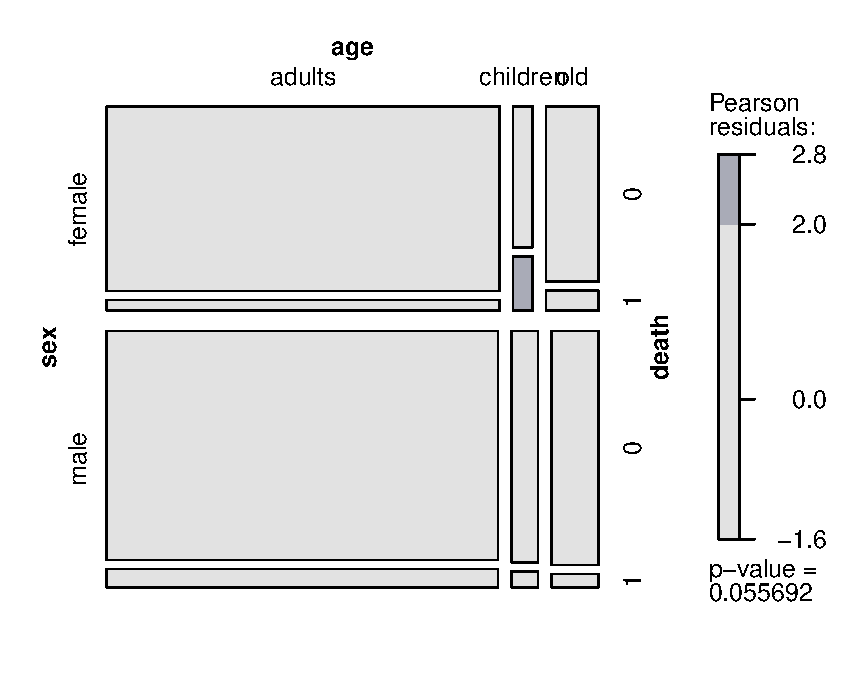
\includegraphics[width=2.3cm]{e3.eps}
  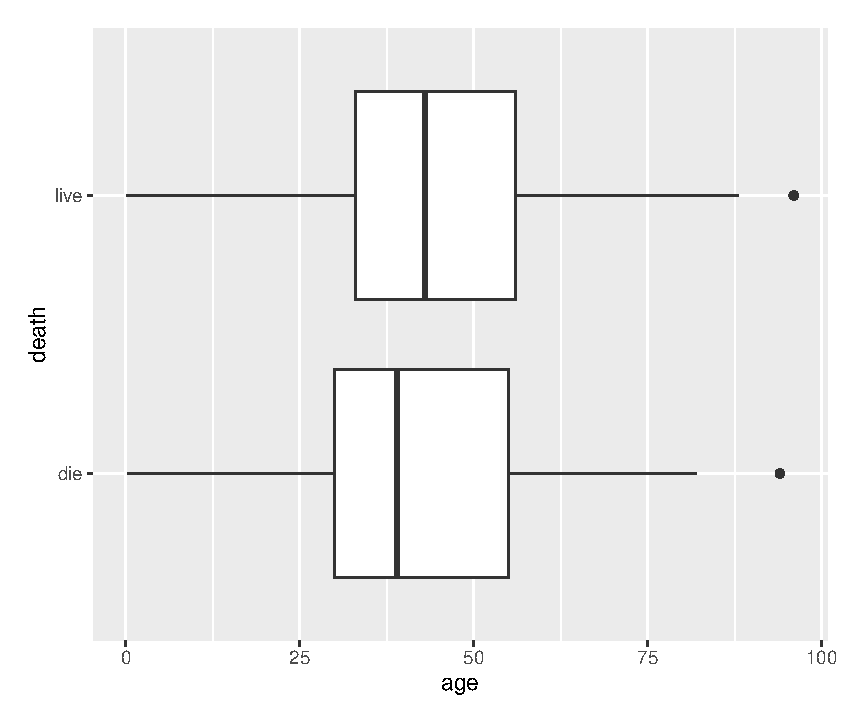
\includegraphics[width=2.3cm]{e4.eps}
    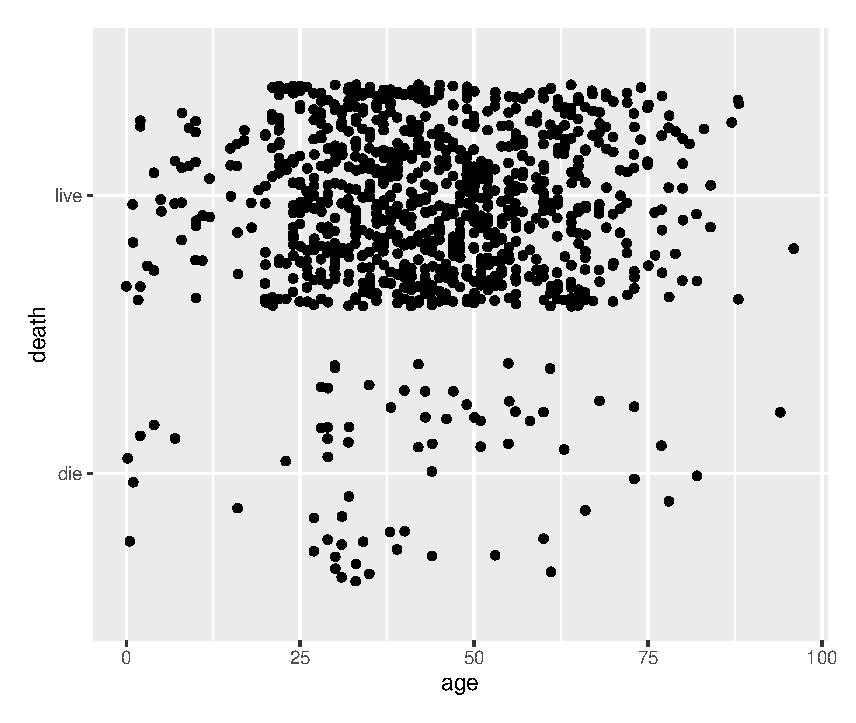
\includegraphics[width=2.3cm]{e5.eps}
\item {\bf1/\ \ The type of three diagrams:}
	\begin{enumerate}
\item Mosaic plot
\item Box plot(ggplot2)
\item Scatter diagram by gplot (ggplot2)
	\end{enumerate}
\end{minipage}
\begin{minipage}[c]{8.35cm}
\begin{enumerate}
{\bf 2/\ \ Analysis}
\\The {\bf first} graph shows that the mortality rate is slightly lower in female adults .\\ The old have higher mortality rates than adults, with children being the highest, but its residuals are too large to be accepted.
\\The {\bf second} and the {\bf third} graphs show that most of the sufferers and the dead are adults, but the mortality rate among adults is the lowest .(Guess:There are fewer children and the elderly)
\\\item {\bf Additional information}
\\Graph1:Children(0-18),Adults(19-65),Old(65+)
\end{enumerate}
\end{minipage}
	
  \vspace{0.5em}
  }

%%%%%%%%%%%%%%%%%%%%%%%%%%%%%%%%%%%%%%%%%%%%%%%%%%%%%%%%%%%%%%%%%%%%%%%%%%%%%%
  \headerbox{LINEAR MODEL(3)(Analysis)}{name=discrete,column=3,row=0}{
\begin{minipage}[c]{2cm}
{\bf \smaller{residuals graph }}
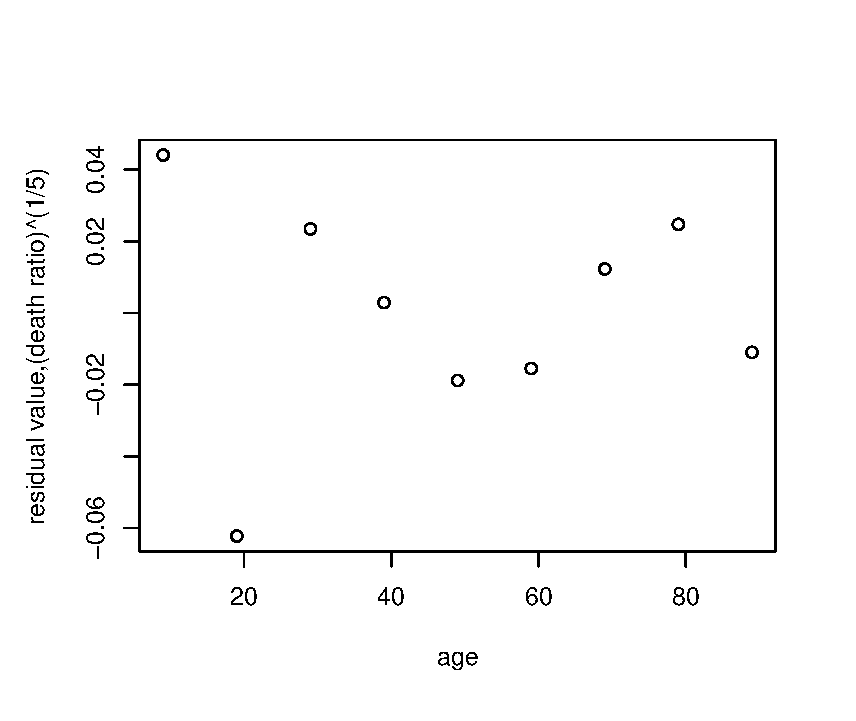
\includegraphics[width=1.65cm]{e8.eps}
\centering{\bf{\smaller{boxplot}}}
\includegraphics[width=1.65cm]{e9.eps}
\end{minipage}
\begin{minipage}[c]{6cm}
\\{\smaller	{\bf ANALYSIS}
\\1.Most of the points are randomly distributed around 0,this is the evidence to the normal distribution.
\\2.There is no outlier,\ and the most of the points are within 0.04 and -0.06 .
\\{\bf SUMMARY:}
\\So the fit is good enough.}
\end{minipage}
  \vspace{0.2em}
  }


%%%%%%%%%%%%%%%%%%%%%%%%%%%%%%%%%%%%%%%%%%%%%%%%%%%%%%%%%%%%%%%%%%%%%%%%%%%%%%
 \headerbox{CONCLUSIONS\& INFORMATION}{name=continuous,column=3,below=discrete}{
{\bf BY DATA1\&2}
\\1.Males are more likely to die than females.
\\2.The relationship between age and mortality is more obvious. The rate increases with age.(opposite with many other infectious diseases[1])
\\{\bf INFORMATION IN INTERNET}[4]
\\\begin{minipage}[c]{2.2cm}
\includegraphics[width=1.95cm]{p1.png}
\end{minipage}
\begin{minipage}[c]{5.8cm}
{\smaller 1.Men have a higher risk of death than women.
\\2.The death rate increases with age in a curved line(similar with the result in data2)}
\end{minipage}
  \vspace{0.2em}
  }




%%%%%%%%%%%%%%%%%%%%%%%%%%%%%%%%%%%%%%%%%%%%%%%%%%%%%%%%%%%%%%%%%%%%%%%%%%%%%
\headerbox{LINEAR MODEL(1)}{name=axioms,column=1,below=plots}{
\begin{minipage}[c]{2.5cm}
{\bf Graph of death ratio $\sim$ age}
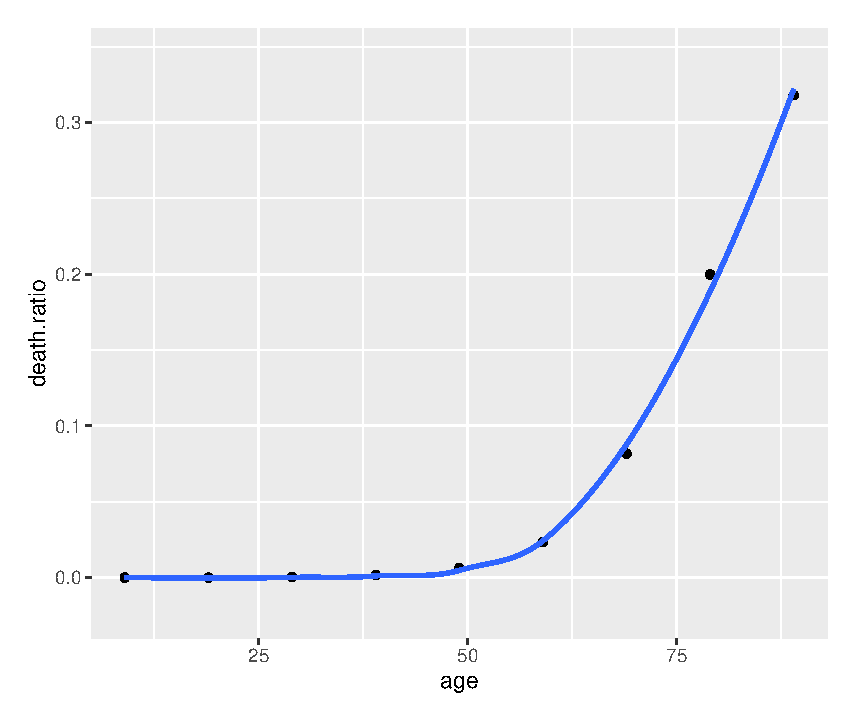
\includegraphics[width=2.5cm]{e6.eps}
\end{minipage}
\begin{minipage}[c]{5.1cm}
Use the data2 on confirmed cases and deaths per 100,000 men and women in the population.[3]
\\Using ggplot2,\ draw a scatter plot and fit the curve.
\\$$Death Ratio=\frac{confirmed\ \ deaths}{confirmed\ \ cases}$$
\end{minipage}
  \vspace{0.2em}
  }

%%%%%%%%%%%%%%%%%%%%%%%%%%%%%%%%%%%%%%%%%%%%%%%%%%%%%%%%%%%%%%%%%%%%%%%%%%%%%
\headerbox{LINEAR MODEL(2)}{name=cond,column=2,below=plots}{
\begin{minipage}[c]{3.5cm}
Using Linear Regression method.
\\Fitting a linear model.
\end{minipage}
\begin{minipage}[c]{4cm}
\centerline{\large{{\bf ${\bf (death\ ratio)}^{\bf \frac{1}{5}}$}{\bf$\sim$ }{\bf age}}}%
\\
 \centering
\includegraphics[width=4cm]{e7.eps}
\end{minipage}
 }

%%%%%%%%%%%%%%%%%%%%%%%%%%%%%%%%%%%%%%%%%%%%%%%%%%%%%%%%%%%%%%%%%%%%%%%%%%%%%%
\headerbox{THE ERROR ANALYSIS}{name=concl,column=3,below=continuous}{
	{\smaller The results of two data sets are slightly different from some information on the Internet, and the first has a higher child mortality rate than the second group.
\\The second is more consistent with expectations.
\\{\bf Analysis:}
\\1.The Mosaic plot in data1 shows that the death ratio in children is not in the range of acceptance,so it should be questioned. 
\\2.The mortality rate changes with time[1], but these datas end at different time(2/29/2020,6/3/2020).
\\3.Data1 misses many datas, more than 12,000 data were deleted, It may cause errors.}
\vspace{0.2em}
	}
	
%%%%%%%%%%%%%%%%%%%%%%%%%%%%%%%%%%%%%%%%%%%%%%%%%%%%%%%%%%%%%%%%%%%%%%%%%%%%%%
  \headerbox{REFERENCES}{name=references,column=3,above=bottom}{
  \smaller
    \vspace{0.97em}
    \bibliographystyle{plain}
    \renewcommand{\section}[2]{\vskip -1.8em}
      \begin{thebibliography}{1}\itemsep=-0.3em
      \setlength{\baselineskip}{1em}
      \bibitem{stir}
       Max Roser, Hannah Ritchie, Esteban Ortiz-Ospina and Joe Hasell.\textit{$Coronavirus Pandemic (COVID-19)$} Available from
: https://ourworldindata.org/coronavirus[Accessed 11th June 2020].
      \bibitem{ross}
       Aadhil Imam.\textit{$COVID19_open_line_list.csv$}
       Available from: https://github.com/aadhil96/covid19\_analysis\_and\_predic\\tion/blob/master/COVID19\_open\_line\_list.csv[Accessed 23rd March 2020]
	\bibitem{grimmett}
			Sliver District.\ \textit{$COVID-19: Data  disaggregated by  age and  sex$}.Available from: https://globalhealth5050.org/covid19/age-and-sex-data/\#1589893214590-52bd08c3-f1e9
			\bibitem{grimmett.}
    			Alexander Yuryatin.\textit{$COVID-19 case fatality-derived risk of death adjusted by age and gender$} Available from:https://zenodo.org/record/3787931\#.Xt4iWp4zYXo\ [Accessed 7th May 2020]
      \end{thebibliography}
  }
%%%%%%%%%%%%%%%%%%%%%%%%%%%%%%%%%%%%%%%%%%%%%%%%%%%%%%%%%%%%%%%%%%%%%%%%%%%%%%
  
\end{poster}

\end{document}
